\documentclass[10pt]{beamer}
\usepackage{amsmath}
\usepackage{mathtools}
\usepackage{multimedia}
\usepackage{hyperref}


\usefonttheme{professionalfonts} % using non standard fonts for beamer
\usefonttheme{serif} % default family is serif
%\documentclass[12pt]{beamerthemeSam.sty}
\usepackage{epsf}
%\usepackage{pstricks}
%\usepackage[orientation=portrait,size=A4]{beamerposter}
\geometry{paperwidth=160mm,paperheight=120mm}
%DT favorite definitions
\def\LL{\left\langle}	% left angle bracket
\def\RR{\right\rangle}	% right angle bracket
\def\LP{\left(}		% left parenthesis
\def\RP{\right)}	% right parenthesis
\def\LB{\left\{}	% left curly bracket
\def\RB{\right\}}	% right curly bracket
\def\PAR#1#2{ {{\partial #1}\over{\partial #2}} }
\def\PARTWO#1#2{ {{\partial^2 #1}\over{\partial #2}^2} }
\def\PARTWOMIX#1#2#3{ {{\partial^2 #1}\over{\partial #2 \partial #3}} }

\def\rightpartial{{\overrightarrow\partial}}
\def\leftpartial{{\overleftarrow\partial}}
\def\diffpartial{\buildrel\leftrightarrow\over\partial}

\def\BS{\bigskip}
\def\BC{\begin{center}}
\def\EC{\end{center}}
\def\BN{\begin{enumerate}}
\def\EN{\end{enumerate}}
\def\BI{\begin{itemize}}
\def\EI{\end{itemize}}
\def\BE{\begin{displaymath}}
\def\EE{\end{displaymath}}
\def\BEA{\begin{eqnarray*}}
\def\EEA{\end{eqnarray*}}
\def\BNEA{\begin{eqnarray}}
\def\ENEA{\end{eqnarray}}
\def\EL{\nonumber\\}

\newcommand{\etal}{{\it et al.}}
\newcommand{\gbeta}{6/g^2}
\newcommand{\la}[1]{\label{#1}}
\newcommand{\ie}{{\em i.e.\ }}
\newcommand{\eg}{{\em e.\,g.\ }}
\newcommand{\cf}{cf.\ }
\newcommand{\etc}{etc.\ }
\newcommand{\atantwo}{{\rm atan2}}
\newcommand{\Tr}{{\rm Tr}}
\newcommand{\dt}{\Delta t}
\newcommand{\op}{{\cal O}}
\newcommand{\msbar}{{\overline{\rm MS}}}
\def\chpt{\raise0.4ex\hbox{$\chi$}PT}
\def\schpt{S\raise0.4ex\hbox{$\chi$}PT}
\def\MeV{{\rm Me\!V}}
\def\GeV{{\rm Ge\!V}}

%AB: my color definitions
%\definecolor{mygarnet}{rgb}{0.445,0.184,0.215}
%\definecolor{mygold}{rgb}{0.848,0.848,0.098}
%\definecolor{myg2g}{rgb}{0.647,0.316,0.157}
\definecolor{A}{rgb}{1.0,0.3,0.3}
\definecolor{B}{rgb}{0.0,1.0,0.0}
\definecolor{C}{rgb}{1.0,1.0,0.0}
\definecolor{D}{rgb}{0.5,0.5,1.0}
\definecolor{E}{rgb}{0.7,0.7,0.7}
\definecolor{abtitlecolor}{rgb}{1.0,1.0,1.0}
\definecolor{absecondarycolor}{rgb}{0.0,0.416,0.804}
\definecolor{abprimarycolor}{rgb}{1.0,0.686,0.0}
\definecolor{Red}           {rgb}{1,0.4,0.4}
\definecolor{Yellow}           {rgb}{1,1,0.0}
\definecolor{Grey}          {cmyk}{.7,.7,.7,0}
\definecolor{Blue}          {cmyk}{1,1,0,0}
\definecolor{Green}         {cmyk}{1,0,1,0}
\definecolor{Brown}         {cmyk}{0,0.81,1,0.60}
\definecolor{Silver}        {rgb}{0.95,0.9,1.0}
\definecolor{Sky}           {rgb}{0.07,0.0,0.2}
\definecolor{Darkbrown}     {rgb}{0.4,0.3,0.2}
\definecolor{40Gray}        {rgb}{0.4,0.4,0.5}
\usetheme{Madrid}


\setbeamercolor{normal text}{fg=Silver,bg=Sky}

%AB: redefinition of beamer colors
%\setbeamercolor{palette tertiary}{fg=white,bg=mygarnet}
%\setbeamercolor{palette secondary}{fg=white,bg=myg2g}
%\setbeamercolor{palette primary}{fg=black,bg=mygold}
\setbeamercolor{title}{fg=abtitlecolor}
\setbeamercolor{frametitle}{fg=abtitlecolor}
\setbeamercolor{palette tertiary}{fg=white,bg=Darkbrown}
\setbeamercolor{palette secondary}{fg=white,bg=absecondarycolor}
\setbeamercolor{palette primary}{fg=white,bg=40Gray}
\setbeamercolor{structure}{fg=abtitlecolor}

\setbeamerfont{section in toc}{series=\bfseries}

%AB: remove navigation icons
\beamertemplatenavigationsymbolsempty
\title[Science and its imitators]{
  \textbf {Science and its imitators}}


\author [Astronomy 101]{Astronomy 101\\Syracuse University, Fall 2018\\Walter Freeman}

\date{\today}

\begin{document}

\frame{\titlepage}

\frame{
``[T]he imagination of nature is far, far greater than the imagination of man (sic). For instance, how much more remarkable it is for us to be stuck -- half of us upside down -- by a mysterious attraction, to a spinning ball that has been swinging in space for billions of years, than to be carried on the back of an elephant supported on a tortoise swimming in a bottomless sea.

\bigskip

For instance, I stand at the seashore, alone, and start to think.

\smallskip

There are the rushing waves, mountains of molecules, each stupidly minding its own business, trillions apart, yet forming white surf in unison.

\smallskip


Ages on ages, before any eyes could see, year after year, thunderously pounding the shore as now.

\smallskip


For whom, for what? On a dead planet, with no life to entertain.

\smallskip


Never at rest,  tortured by energy, wasted prodigiously by the sun, poured into space. A mite makes the sea roar.


\smallskip

Deep in the sea, all molecules repeat the patterns of one another till complex new ones are formed. They make others like themselves, and a new dance starts.

\smallskip


Growing in size and complexity: living things, masses of atoms, DNA, protein... dancing a pattern ever more intricate.

\medskip


Out of the cradle onto the dry land, here it is standing: atoms with consciousness,  matter with curiosity.

\smallskip


Stands at the sea, wonders at wondering: I, a universe of atoms, an atom in the universe.''

\begin{flushright}
--Richard Feynman (again), from {\it The Value of Science} (1955)
\end{flushright}
}


\frame{\frametitle{\textbf{Announcements}}
\Large
\BI
\item Exam answers sent over to OIRA for grading today
\item Hopefully we'll get the results tomorrow and I can post them over the weekend
\pause
\item Lab 6 prelab will be finished tonight and posted, and put in the Clinic
\item Paper 2 will be assigned today
\EI
}

\frame{\frametitle{\textbf{Paper 2}}
\Large
\BC
You have two options for this paper:
\EC

\BI
\item Scientific ethics: write about a case where scientific ethics ran off the rails, or an issue where scientific inquiry must
navigate an ethical minefield 

\BS\pause

\item Archaeoastronomy: write about the astronomical practice of a historical culture of your choice
\EI
}

\frame{\frametitle{\textbf{The nature of science}}

\large

The discoveries of Kepler, Galileo, and Newton did more than explain the solar system.

\bigskip

They merged disciplines that had been separate since the time of the Greeks:

\BI
\item Natural philosophy: ``what is the truth of Nature?'' (truth-seeking)
\item Astronomy: ``Where can I find Mars next week?'' (practical applications)
\EI

\bigskip
Newton brought us into the age of {\it astrophysics} -- possibly the first true {\it science}. What's that mean?

\pause

\BI
\item Truth in precision
\item Synergy between truth-seeking and practical observation
\item Synergy between theory and experiment
\BI
\item Theory: ``Use things we've already observed to design a model''
\item Exp't: ``Carefully choose observations to make to inform/test models''
\EI
\EI
}

\frame{\frametitle{\textbf{The scientific method}}
\Large
\begin{enumerate}
\item ``Huh, that is interesting -- I wonder how it works?''
\item Develop a {\it model}: a picture that explains as much as you can
\item Compare the predictions of your model to real-world observations
\pause
\BI
\item Partial agreement: can we refine the model? (Copernicus)
\item Complete disagreement: Tear it up and go back to (1)
\EI
\item Model agrees with observations so far: It's a useful {\it theory}
\pause
\item Does the model predict new things not yet observed?
\item Design observations to test for them (experiments!)
\BI
\item Partial agreement: can we refine the model?
\item Complete disagreement: Tear it up and go back to (1)
\EI
\pause
\item Body of supporting evidence grows
\item Continually seek to expand the {\it scope} of the model with more observations
\end{enumerate}
}

\frame{\frametitle{\textbf{An example: Mechanics}}
\large
\BI
\item ``I wonder how things move?'' --Everyone
\item Newton's model of mechanics
\item Tested continually as engineering developed in the Industrial Revolution
\item ... always found to hold, precisely, for any machine we built \pause

\bigskip

\item Expanding the scope:
\BI
\normalsize
\item Atoms and molecules
\item ``I wonder how heat works?'' --Everyone
\item ``Maybe it's just atoms jiggling around?'' --Boltzmann
\item {\color{Red}It turns out we can do a lot more with $F=ma$ than we thought!} 
\EI
\pause

\bigskip

\item What about inside the atom?
\BI
\normalsize
\item $F=ma$ not the whole picture -- need to revise ideas of ``position'', ``acceleration'', etc.
\item Model right, assumptions and language needed modification
\item Birth of quantum mechanics
\EI\pause

\bigskip

\item What about gravity very close to big things?
\BI
\normalsize
\item Scope of Newton's gravity had to be modified
\item Newtonian gravity only right for small accelerations
\item Einstein: ``I think I have a new model''
\item Newtonian gravity still correct within its scope
\EI
\EI
}

\frame{\frametitle{\textbf{Attributes of science }}
\Large \BC

What things do scientific explanations have in common?

\EC

\bigskip

\BI
\pause
\item ``We can understand this thing!'' -- explanations must be {\color{Red} natural}
\pause
\item Models try to be {\color{Red}universal}
\pause
\item Predictions are {\color{Red}testable}
\pause
\item Studies try to be {\color{Red}objective} (this is hard -- statistics helps)
\pause
\item Studies are at least in principle {\color{Red}replicable} -- anyone can redo them

\bigskip \pause

\item Scientific explanations are {\color{Red}not anthropocentric} -- they don't give humans (or Earth) a special role
\EI
}

\frame{\frametitle{\textbf{The natural worldview}}
\Large
Science doesn't attempt to answer everything, only:

\BI
\item ... what is the Universe made of?
\item ... how does it work?
\item Questions like: ``if I do this, what will happen?''
\EI

\bigskip\pause

It doesn't address questions like...

\BI
\item ``What {\it should} we do here?''
\item ``What does it mean to be a good person?''
\pause
\item ``How should we imagine our place in the world?''
\EI

\bigskip\pause

The natural, non-anthropocentric view {\it does} influence our outlook, though...}

\frame{\frametitle{\textbf{Scientific integrity}}
\large
``But this long history of learning how not to fool ourselves--of
having utter scientific integrity--is, I'm sorry to say, something
that we haven't specifically included in any particular course that
I know of. We just hope you've caught on by osmosis.

The first principle is that you must not fool yourself--and you are
the easiest person to fool. So you have to be very careful about
that. After you've not fooled yourself, it's easy not to fool other
scientists. You just have to be honest in a conventional way after
that.

\medskip
\BC ... \EC
\medskip

I'm talking about
a specific, extra type of integrity that is not lying, but bending
over backwards to show how you are maybe wrong, that you ought to
have when acting as a scientist.

\medskip
\BC ... \EC
\medskip

One example of the principle is this: If you've made up your mind
to test a theory, or you want to explain some idea, you should
always decide to publish it whichever way it comes out. If we only
publish results of a certain kind, we can make the argument look
good. We must publish both kinds of results.''

\bigskip

\begin{flushright} --Feynman, commencement address at Caltech, 1974\end{flushright}
}


\frame{

\large

There's an entire discipline of mathematics designed to, in an objective way, examine what results mean: {\color{Red} statistics.}

\bigskip

But it's only as honest as the people wielding it: \url{https://xkcd.com/882/}

}


\frame{\frametitle{\textbf{Science: a powerful tool}}
\Large \BC
This synergistic enterprise has been behind a vast amount of progress for humanity in the last 350 years.
\EC
\bigskip
\bigskip

As with anything powerful, this process can be corrupted:

\BI
\item{Confirmation bias / placebo effect}
\item{Ulterior motives: young-earth creationism, climate science, politicization}
\item Profit motive: vaccines causing autism
\item Publication bias (jellybeans!)
\item Artificially limited scope (some psych studies)
\EI
}

\frame{\frametitle{\textbf{Science vs. pseudoscience}}
\BC\Large
Often people adopt the trappings of science to give nonscientific ideas a veneer of validity.
This is called ``pseudoscience'' -- fake science.
\EC

\begin{columns}

\column{0.5\textwidth}
\color{Green}
\Large \BC Science \EC
\large
\BI
\item Universal models
\item Natural principles
\item Testable predictions
\item Not anthropocentric
\item Replicable results
\item Self-skepticism
\EI

\column{0.5\textwidth}
\color{Red}
\Large \BC Pseudoscience\EC
\large
\BI
\item Singular events
\item Supernatural explanations
\item Untestable predictions
\item Different rules for people
\item Results defy replication
\item Self-promotion
\EI
\end{columns}
}

\frame{
\Large
\BC
What would you like to talk about?
\EC

\BI
\item Astrology
\item Economics and integrity
\item Ghosts and such
\item Homeopathy vs. desensitization therapy
\item Climate change
\item Genetically-modified crops and statistics
\item Vaccination
\item ESP / telepathy
\item Exterrestrial life
\item Radioactive medicine
\item Drug testing
\item Medical marijuana
\item Scientific integrity more broadly
\item Something else...
\EI
}

\frame{

\large
``Our time is distinguished by wonderful achievements in the fields of scientific understanding and the technical application of those insights. Who would not be cheered by this? But let us not forget that human knowledge and skills alone cannot lead humanity to a happy and dignified life. Humanity has every reason to place the proclaimers of high moral standards and values above the discoverers of objective truth. What humanity owes to personalities like Buddha, Moses, and Jesus ranks for me higher than all the achievements of the enquiring and constructive mind.
What [they] have given us we must guard and try to keep alive with all our strength if humanity is not to lose its dignity, the security of its existence, and its joy in living.''

\bigskip

\begin{flushright}--Albert Einstein, 1937\end{flushright}


\bigskip\pause
\bigskip
\bigskip
\bigskip

``Tell your son to stop trying to fill your head with science, for to fill your heart with love is enough!''

\bigskip

\begin{flushright}--Richard Feynman, 1981\end{flushright}

}

\frame{
\BC
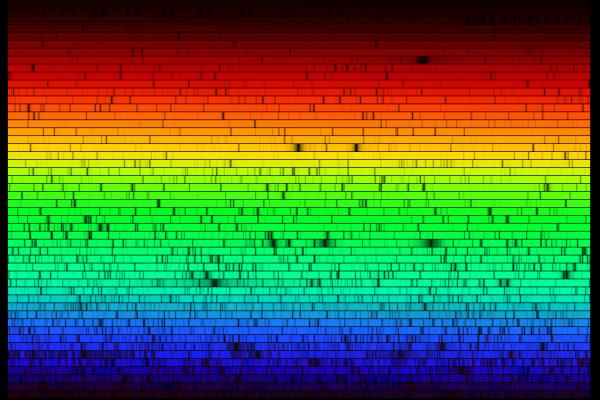
\includegraphics[width=0.9\textwidth]{solarspectrum.jpg}
\large

This is a ``picture'' of the Sun. What can we learn from it?
\EC
}

\frame{

\large
\BC
How much of the light in this room can you see?\EC

\BS\BS
\Large
\color{A}A: All of it\\
\color{B}B: Most of it \\
\color{C}C: Around a quarter of it\\
\color{D}D: Not much of it at all\\
}

\frame{
\large
\BC
\large
How much of the sound in this room can you hear?\EC
\Large
\BS\BS

\color{A}A: All of it\\
\color{B}B: Most of it \\
\color{C}C: Around a quarter of it\\
\color{D}D: Not much of it at all\\
}

\frame{
\large
\BC
Sounds can have a spectrum of frequencies and wavelengths, 
and we can only perceive a piece of that spectrum.

\BS\BS\pause

\BS

In the same way {\it light} has a spectrum of frequencies/wavelengths, 
and our eyes only perceive a tiny fraction of that spectrum.

\color{Red}
When we say ``light'', we mean {\it all} wavelengths, not just the 
ones we can see!
\EC
}

\frame{\frametitle{\bf The electromagnetic spectrum}

\BC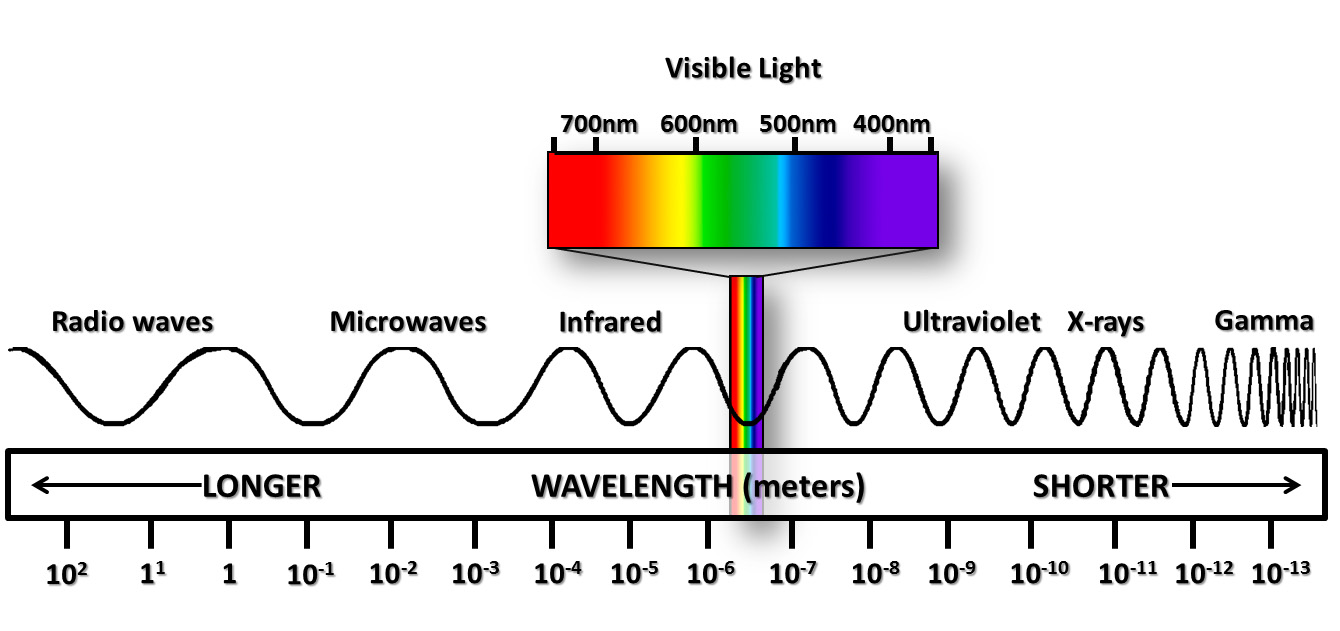
\includegraphics[width=0.8\textwidth]{linear-spectrum.jpg}

\BS

There is an enormous range of ``colors'' of light out there!\EC

\BS\BS

What's this ``sound'' like?

\pause
\BS
{Music: ``The Blood of Cu Chulainn'', from the soundtrack to {\it Boondock Saints} (Jeff Danna, 1999)}

\BS\pause

We can learn far more about what's going on in the orchestra if we 
have the whole spectrum, rather than just a piece!
}

\frame{
\BC
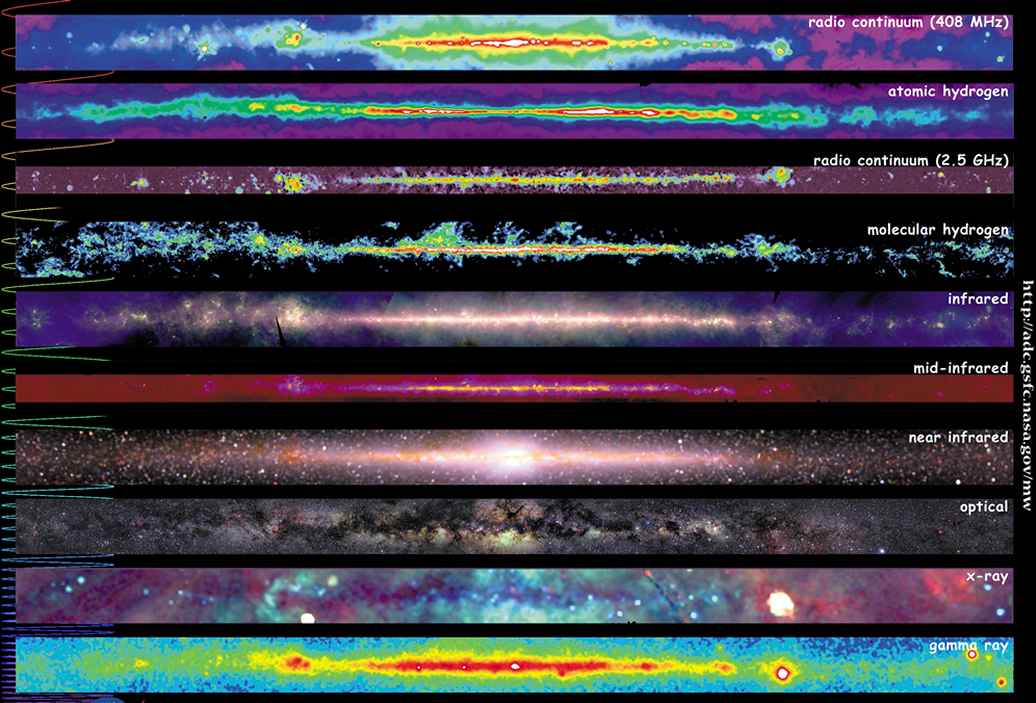
\includegraphics[height=0.9\textheight]{mwmw.jpg}
\EC
}



\frame{\frametitle{\bf{An illuminating story}}

In the late 19th century, the laws of electromagnetism looked like this:

\BI
\item Electric fields exert a force on electric charges
\item Magnetic fields exert a force on {\it moving} electric charges
\EI

\bigskip

We know this thanks in large part to the work of Michael Faraday, who
famously wasn't good at algebra and drew pictures of fields.

\bigskip

Where do these fields come from?

\BI
\item Electric charges make electric fields
\item Moving electric charges make magnetic fields
\item Changing magnetic fields make electric fields
\pause
\item {\color{Red} Changing electric fields make magnetic fields}
\EI
}

\frame{\frametitle{\bf{An illuminating story}}

\BI
\item Electric charges make electric fields
\item Moving electric charges make magnetic fields
\item Changing magnetic fields make electric fields
\item {\color{Red} Changing electric fields make magnetic fields}
\EI

\BS

Last law added by James Clerk Maxwell in the 1860's, and it has
a surprising consequence:

\BS
\BI
\item{Changing electric field makes a magnetic field}
\pause \item ... which makes a magnetic field ...
\pause \item ... which makes an electric field further away ...
\pause \item This leads to a traveling electromagnetic disturbance: an {\it electromagnetic wave}.
\EI
}

\frame{\frametitle{\bf{An illuminating story}}

Maxwell calculated that these electromagnetic waves traveled at
around 300 million meters per second.

\BS

Independently, light had been measured to travel at 300 million
meters per second some years prior.

\BS \pause

So ... if this electromagnetic wave travels at the speed of
light, perhaps it {\it is} light?

\BS

In the history of science, sometimes theory gets ahead of experiment -- like in the discovery of the nature of light.
}



\end{document}
